\documentclass[nobib]{tufte-handout}

\title{Lecture 2: Eulerianity, simple graphs, and subgraphs $\cdot$ 1MA020}

\author[Vilhelm Agdur]{Vilhelm Agdur\thanks{\href{mailto:vilhelm.agdur@math.uu.se}{\nolinkurl{vilhelm.agdur@math.uu.se}}}}

\date{24 October 2023}


%\geometry{showframe} % display margins for debugging page layout

\usepackage{graphicx} % allow embedded images
  \setkeys{Gin}{width=\linewidth,totalheight=\textheight,keepaspectratio}
  \graphicspath{{graphics/}} % set of paths to search for images
\usepackage{amsmath}  % extended mathematics
\usepackage{booktabs} % book-quality tables
\usepackage{units}    % non-stacked fractions and better unit spacing
\usepackage{multicol} % multiple column layout facilities
\usepackage{lipsum}   % filler text
\usepackage{fancyvrb} % extended verbatim environments
  \fvset{fontsize=\normalsize}% default font size for fancy-verbatim environments

\usepackage{color,soul} % Highlights for text

% Standardize command font styles and environments
\newcommand{\doccmd}[1]{\texttt{\textbackslash#1}}% command name -- adds backslash automatically
\newcommand{\docopt}[1]{\ensuremath{\langle}\textrm{\textit{#1}}\ensuremath{\rangle}}% optional command argument
\newcommand{\docarg}[1]{\textrm{\textit{#1}}}% (required) command argument
\newcommand{\docenv}[1]{\textsf{#1}}% environment name
\newcommand{\docpkg}[1]{\texttt{#1}}% package name
\newcommand{\doccls}[1]{\texttt{#1}}% document class name
\newcommand{\docclsopt}[1]{\texttt{#1}}% document class option name
\newenvironment{docspec}{\begin{quote}\noindent}{\end{quote}}% command specification environment

\include{mathcommands.extratex}

\begin{document}

\maketitle% this prints the handout title, author, and date

\begin{abstract}
\noindent
We formalize the ideas we started with in the first exercise session, giving a proof of Euler's result on Eulerian circuits. We then make some more definitions about simple graphs and subgraphs, and we state some elementary results about these notions.
\end{abstract}

The very first definition we give in this course will actually be of a \emph{multigraph}, not the simple graphs that were our first example.\sidenote[][-0.7cm]{These are of course a type of graph, so we will often just write or say ``graph'' when it is clear from context what type of graph we are referring to, or what we are saying applies to any type of graph.}

\begin{definition}
    A \emph{multigraph} $G$ is a tuple $(V, E)$, consisting of a set $V$ of \emph{vertices}, and a multiset\sidenote[][]{A multiset is just like a set, except an element may occur more than once.} $E$ of \emph{edges}. Each edge is a multiset containing two vertices from $V$, called its \emph{endpoints}. We say two vertices are \emph{adjacent} if there is an edge between them, and a vertex $v$ is \emph{incident} to an edge $e$ if $v \in e$.

    If the same edge occurs more than once in $E$, we say that these edges are \emph{parallel}. If the two endpoints of an edge are equal, we call it a \emph{loop}.

    Unless explicitly stated, we always assume that both $V$ and $E$ are finite sets. Otherwise, we say the graph is \emph{infinite}.\sidenote[][]{It may sometimes be the case that our proofs work without modification also for infinite graphs -- thinking about whether they do may be a useful thing to do when reading the proofs, to understand them better.}
\end{definition}

Next, continuing to formalize the things we learned thinking about the bridges of Königsberg, let us define what a walk is.

\begin{definition}
    Let $G = (V, E)$ be a multigraph. A \emph{walk} of length $k$ is a sequence of $k+1$ vertices $v_0 v_1 v_2\ldots v_k$ and a sequence of $k$ edges\sidenote[][]{So the length of a walk is the number of edges, not the number of vertices.} $e_1e_2\ldots e_k$ such that $e_i = \{v_{i-1}, v_i\}$ for all $i$. A \emph{trail} is a walk that uses no edge twice, and a \emph{path} is a walk that uses no vertex twice. A \emph{circuit} is a trail where the first and last vertices coincide, and a \emph{cycle} is a circuit where these are the only vertices that coincide.
\end{definition}

\begin{figure}
    \centering
    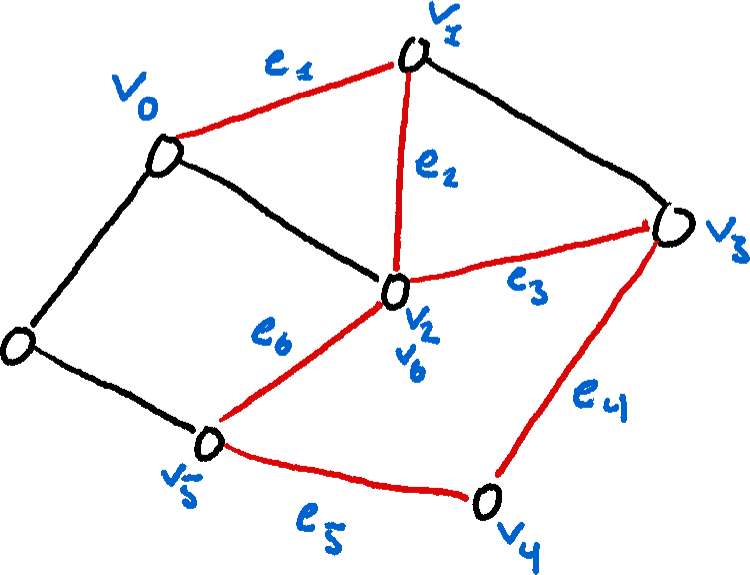
\includegraphics[width=0.7\textwidth]{graphics/L2_eulerianity_subgraphs/walk_in_graph.png}
    \caption[][0cm]{A walk in a graph, which is a trail but not a path.}
    \label{fig:walk_in_graph}
\end{figure}

We have one example of a walk in Figure \ref{fig:walk_in_graph} -- it does not repeat any of the edges, so it is a trail, but it repeats the central vertex we have labelled with both $v_2$ and $v_6$, so it is not a path.

Having introduced walks, we can give a definition of another very natural property, namely connectedness.\sidenote[][]{You've probably already seen the notion of connectedness of a subset of $\R^2$ in a calculus course, and if you've looked at other geometry it appears there as well. This is the same notion, just discretized.}

\begin{definition}
  We say that a graph $G$ is \emph{connected} if there is, for any two vertices $u, v \in G$, a walk from $u$ to $v$. We say that two vertices in a graph are connected to each other if there is a walk between them.

  Notice that there is a trivial ``lazy'' walk connecting every vertex to itself, so the relation of connectedness is an equivalence relation. The equivalence classes of this equivalence relation are called the \emph{connected components} of the graph.\sidenote[][]{We could equivalently have defined the connected components as the maximal connected subgraphs of the graph -- when we get to a formal definition of subgraph, think about why this is true.}
\end{definition}

Let us now define the thing we were studying when we thought about the bridges of Königsberg.

\begin{definition}
  An \emph{Eulerian trail} is a trail that uses every edge in the graph exactly once -- if additionally it has the same starting and ending vertex, we call it an \emph{Eulerian circuit}. If there is an Eulerian circuit in a graph, we call the graph \emph{Eulerian}.
\end{definition}

The problem we were studying was thus to find a simple condition for when a multigraph is Eulerian. The condition we found\sidenote[][]{Hopefully.} involved the number of edges incident to a vertex, so let us also give this notion a name.

\begin{definition}
  The \emph{degree} of a vertex $v$, denoted $d_v$, is the number of edges a vertex is incident to, with loops counted twice.
\end{definition}

We now have all the language we need to formally state and prove the theorem that started graph theory all those nearly three hundred years ago.

\begin{theorem}[Euler (1736)]
  A finite connected multigraph is Eulerian if and only if all its vertices have even degree.
\end{theorem}

%\bibliography{references}
%\bibliographystyle{plainnat}

\end{document}
